\section{Using the New Measure}
\label{sec:replications}

We have shown that our measure, the DOE score, predicts international dispute outcomes better than the current state of the art, the capability ratio.
But most recent studies of conflict do not aim to predict how disputes will end.
They focus on other dependent variables, and they usually only treat the capability ratio (or other functions of raw capabilities) as a control.
In this section, we investigate how well the DOE score performs as a replacement for the capability ratio in this more typical setting.
First, we replicate 18 recent empirical models of various international phenomena, finding that these models usually fit and predict better when we replace CINC-based measures with DOE scores.
After that, we provide some advice to practitioners on how to decide which measure---or measures---to include.

\subsection{Replication Analysis}

International relations scholars often control for the capability ratio as a proxy for expected outcomes when modeling dependent variables besides who wins, such as the onset or escalation of a dispute.
We have shown that the DOE score is a better proxy than the capability ratio, but it does not follow immediately that it is a better control variable in studies of conflict more generally.
Can we improve on these analyses---i.e., do our regressions fit the data better---if we replace the capability ratio with our new measure?
To address this question, we replicate 18 recent analyses of conflict using DOE scores in place of the capability ratio or other functions of CINC scores.
On the whole, we see that the models with DOE scores tend to have better in- and out-of-sample fit, though not always.

\afterpage{
  \clearpage
  \begin{landscape}
    \begin{table}[h]
      \centering
      \input{tab-replications}
      \caption{
        Summary of results from the replication analysis.
        In-sample goodness of fit is measured by the AIC and the \citet{Vuong:1989uf} test.
        Positive values of the Vuong test statistic indicate that the model with DOE terms fits better than the model with CINC terms, and vice versa for negative values.
        The Vuong test statistic has a standard normal distribution under the null hypothesis of no difference between the models, so values with a magnitude of $1.96$ or greater would lead us to reject the null hypothesis at the $0.05$ significance level.
        Out-of-sample fit is measured by proportional reduction in log loss relative to the null model, as reported in the last two columns.
        We use repeated 10-fold cross-validation to estimate each model's out-of-sample log loss, with 10 repetitions for models indicated by a dagger ($\dag$) and 100 repetitions for all others.
        The null model's log loss is estimated via leave-one-out cross-validation.
      }
      \label{tab:replications}
    \end{table}
  \end{landscape}
}

We constructed the set of replications by looking for empirical analyses of dyad-years (directed or undirected) that included the capability ratio or another function of CINC scores as a covariate.
Each study was published recently in a prominent political science or international relations journal.\footnote{
  For details, see footnote~\ref{fn:replications}.
}
We examined only studies with publicly available replication data.
If we could not reproduce a study's main result or were unable to merge the DOE scores into the replication data (e.g., because of missing dyad-year identifiers), we excluded it from the analysis.
We also excluded studies that employed duration models or selection models, due to conceptual and technical problems with assessing their out-of-sample performance.
Lastly, we excluded studies in which our measure of expected dispute outcomes would be endogenous, namely those whose dependent variable was MID outcomes---the same data we used to construct the DOE scores---or a closely related quantity.
In the end, we were left with the 18 studies listed in Table~\ref{tab:replications}.

For each analysis in our sample, we begin by identifying the main statistical model reported in the paper, or at least a representative one.\footnote{
  When no main model is apparent, our heuristic is to pick one on the log-likelihood--sample size frontier.
  Details of the model chosen from each paper and the functions of CINC and DOE scores used are in the Appendix.
}
We then estimate two models: the original model, and a replicated model where we replace any functions of CINC scores with their natural equivalents in DOE scores.
For example, if the capability ratio is logged in the original model, we log the DOE scores in the replicated model.
As a basic measure of each model's in-sample goodness of fit, we compute the \citet{Akaike:1974ih} Information Criterion,\footnote{
  Because DOE scores are ternary, the replicated models typically have more parameters than their original counterparts.
  Hence we measure in-sample fit with the AIC, which penalizes over-parameterization, rather than the log-likelihood.
}
\begin{displaymath}
  \text{AIC}
  =
  2(\text{number of coefficients}) - 2(\text{log-likelihood}).
\end{displaymath}
The AIC is commonly used in model selection, with lower values representing better fit.
In addition, we compute the \citet{Vuong:1989uf} test of the null hypothesis that the original and replicated models fit equally well.\footnote{
  We employ the standard Bayesian Information Criterion \citep{Schwarz:1978kh} correction to the Vuong test statistic.
}
To estimate each model's out-of-sample fit, we perform repeated 10-fold cross-validation.
Because each study has a discrete dependent variable, we again employ the log loss (equation~\eqref{eq:log-loss}) to measure out-of-sample fit.

Table~\ref{tab:replications} summarizes the results of the replication analysis.
In general, the models that include DOE scores do better than those with CINC scores by both in- and out-of-sample criteria.
Starting with in-sample fit, we see that the DOE model has a lower AIC than the CINC model in 15 of 18 cases.
Moreover, in more than half of those cases (8), under the Vuong test we would reject at the 0.05~significance level the null hypothesis that the models fit equally well.
The difference in fit is also statistically significant in all three cases where the CINC model has a lower AIC.
The results are similar for out-of-sample fit, with the DOE model having a greater proportional reduction in log loss in 14 cases.
The improvement due to using DOE scores is typically modest---about a single percentage point increase in the proportional reduction in log loss.
For context, keep in mind that these studies do not take capability measures as a key theoretical variable of interest.
In each regression, the capability measure is just one of a battery of control variables.
With so much else going on in these models, even a substantial improvement in the quality of the capability measure may lead to just a small increase in overall model fit or predictive power.

With such a small sample of replicated studies, we can only conjecture about why DOE performs better in some cases and worse in others.
We see that the cases where DOE is significantly better according to the Vuong test tend to have large sample sizes---but, then again, the study where it does worst has the largest $N$ in our sample.
In two of the replications where DOE performs worst, namely \citet{Bennett:2006gp} and \citet{Fordham:2008gs}, we see that both specifications include the raw CINC scores alongside or in lieu of the capability ratio.
These terms may be capturing monadic effects that the purely dyadic DOE scores miss.
On the other hand, in the other three analyses that include raw CINC scores \citep{Arena:2009gk,Zawahri:2011iy,Weeks:2012be}, the replication with DOE scores performs better by both AIC and cross-validation loss.

\subsection{Advice to Practitioners}

Seeing as neither the capability ratio nor DOE scores are uniformly better in typical applications, how should empirical scholars choose which one to include in their analysis?
Our main recommendation is a theory-driven approach.
When theory provides no guidance, we recommend either a data-driven approach or dropping capability measures altogether.

\begin{figure}[htp]
  \centering
  % Main document must include
% \usepackage{tikz}  % for the graphics
% \usepackage{etoolbox}  % for the if-then toggles

\providetoggle{cap-to-dv}
\providetoggle{doe-to-dv}

\togglefalse{cap-to-dv}
\toggletrue{doe-to-dv}

% Main document must include
% \usepackage{tikz}  % for the graphics
% \usepackage{etoolbox}  % for the if-then toggles

\providetoggle{cap-to-dv}
\providetoggle{doe-to-dv}

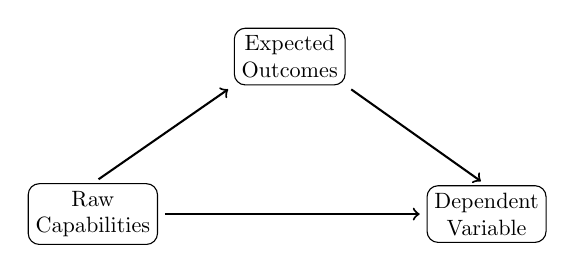
\begin{tikzpicture}[
  var/.style={
    rectangle,
    rounded corners,
    draw=black,
    align=center,
    scale=0.8
    }
  ]
  
  \node[var] (cap) at (0, 0) {Raw\\Capabilities};
  \node[var] (doe) at (2.5, 2) {Expected\\Outcomes};
  \node[var] (dv) at (5, 0) {Dependent\\Variable};

  \path[->, line width=0.75pt] (cap.north) edge[shorten <=0.25em, shorten >=0.25em] (doe.south west);
  \iftoggle{doe-to-dv}{\path[->, line width=0.75pt] (doe.south east) edge[shorten <=0.25em, shorten >=0.25em] (dv.north);}{}
  \iftoggle{cap-to-dv}{\path[->, line width=0.75pt] (cap.east) edge[shorten <=0.25em, shorten >=0.25em] (dv.west);}{}
\end{tikzpicture}

%%% Local Variables:
%%% mode: latex
%%% TeX-master: "doe"
%%% End:


  \caption{
    Raw capabilities only affect the outcome of interest through expectations.
  }
  \label{fig:dag-cap0-doe1}
\end{figure}

If theory suggests that material capabilities only affect the outcome of interest insofar as they shape expectations about how a dispute would end, then DOE scores are the best measure to control for.
Figure~\ref{fig:dag-cap0-doe1} contains a causal graph of this situation.
The clearest examples of theories where only expectations matter come from the formal literature on crisis bargaining.
Take \citeauthor{powell1999}'s~\citeyearpar{powell1999} theory of bargaining in the shadow of power.
War is possible only if the status quo distribution of benefits is far enough from the expected outcome of conflict that at least one state is dissatisfied.
An empirical model derived from this theory should control for DOE scores rather than the capability ratio or other poor proxies for expectations.

\begin{figure}[htp]
  \centering
  % Main document must include
% \usepackage{tikz}  % for the graphics
% \usepackage{etoolbox}  % for the if-then toggles

\providetoggle{cap-to-dv}
\providetoggle{doe-to-dv}

\toggletrue{cap-to-dv}
\toggletrue{doe-to-dv}

% Main document must include
% \usepackage{tikz}  % for the graphics
% \usepackage{etoolbox}  % for the if-then toggles

\providetoggle{cap-to-dv}
\providetoggle{doe-to-dv}

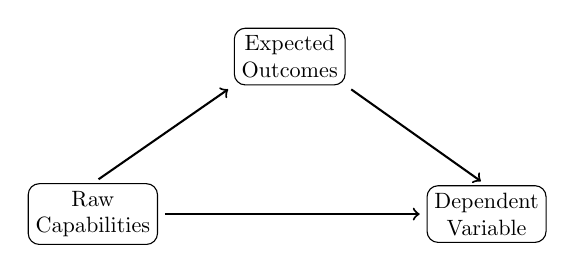
\begin{tikzpicture}[
  var/.style={
    rectangle,
    rounded corners,
    draw=black,
    align=center,
    scale=0.8
    }
  ]
  
  \node[var] (cap) at (0, 0) {Raw\\Capabilities};
  \node[var] (doe) at (2.5, 2) {Expected\\Outcomes};
  \node[var] (dv) at (5, 0) {Dependent\\Variable};

  \path[->, line width=0.75pt] (cap.north) edge[shorten <=0.25em, shorten >=0.25em] (doe.south west);
  \iftoggle{doe-to-dv}{\path[->, line width=0.75pt] (doe.south east) edge[shorten <=0.25em, shorten >=0.25em] (dv.north);}{}
  \iftoggle{cap-to-dv}{\path[->, line width=0.75pt] (cap.east) edge[shorten <=0.25em, shorten >=0.25em] (dv.west);}{}
\end{tikzpicture}

%%% Local Variables:
%%% mode: latex
%%% TeX-master: "doe"
%%% End:


  \caption{
    Raw capabilities affect the outcome of interest both directly and through expectations.
  }
  \label{fig:dag-cap1-doe1}
\end{figure}

If material capabilities affect the outcome both directly and indirectly via expectations, then it would be appropriate to control for both raw capabilities and expected dispute outcomes.
Figure~\ref{fig:dag-cap1-doe1} illustrates this scenario.
For example, imagine an empirical study of ``sinking costs'' via military mobilization in international crises \citep{fearon_signaling_1997}.
The initial movement of peaceful relations into a crisis, as well as early behavior at the bargaining table, might be shaped solely by states' expectations about dispute outcomes.
But if states build up their military as a way to signal resolve, independently of the effect on likely outcomes, then raw capabilities matter too.
When empirically modeling a theory like this, scholars should include both DOE scores and raw capability measures.
The ratio of CINC scores may or may not be the most appropriate way to capture raw capabilities---that, too, depends on the specifics of the theory.

\begin{figure}[htp]
  \centering
  % Main document must include
% \usepackage{tikz}  % for the graphics
% \usepackage{etoolbox}  % for the if-then toggles

\providetoggle{cap-to-dv}
\providetoggle{doe-to-dv}

\toggletrue{cap-to-dv}
\togglefalse{doe-to-dv}

% Main document must include
% \usepackage{tikz}  % for the graphics
% \usepackage{etoolbox}  % for the if-then toggles

\providetoggle{cap-to-dv}
\providetoggle{doe-to-dv}

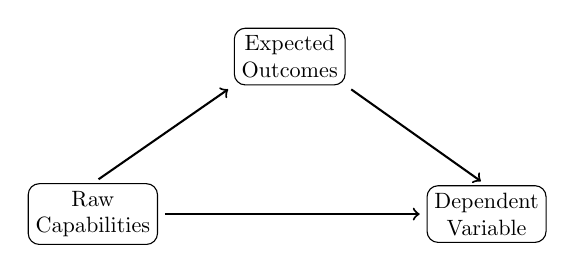
\begin{tikzpicture}[
  var/.style={
    rectangle,
    rounded corners,
    draw=black,
    align=center,
    scale=0.8
    }
  ]
  
  \node[var] (cap) at (0, 0) {Raw\\Capabilities};
  \node[var] (doe) at (2.5, 2) {Expected\\Outcomes};
  \node[var] (dv) at (5, 0) {Dependent\\Variable};

  \path[->, line width=0.75pt] (cap.north) edge[shorten <=0.25em, shorten >=0.25em] (doe.south west);
  \iftoggle{doe-to-dv}{\path[->, line width=0.75pt] (doe.south east) edge[shorten <=0.25em, shorten >=0.25em] (dv.north);}{}
  \iftoggle{cap-to-dv}{\path[->, line width=0.75pt] (cap.east) edge[shorten <=0.25em, shorten >=0.25em] (dv.west);}{}
\end{tikzpicture}

%%% Local Variables:
%%% mode: latex
%%% TeX-master: "doe"
%%% End:


  \caption{
    Raw capabilities directly affect the outcome of interest, but expectations do not.
  }
  \label{fig:dag-cap1-doe0}
\end{figure}

The last possibility to consider is that expectations do not affect the outcome of interest.
In this case, empirical models should only include raw capability measures, not DOE scores.
The clearest example is when the dispute outcome itself is the dependent variable.
First, absent some kind of self-fulfilling prophecy effect, we would expect actual capability holdings to drive outcomes more so than expectations.
Second, because DOE scores are calculated using the dispute outcome data, the DOE scores themselves are endogenous to observed outcomes, and thus should not be included as an independent variable when outcome is the dependent variable.\footnote{
  In principle, this latter problem could be solved, albeit at great computational expense, by only using data for years up to $t-1$ to calculate the DOE score for year~$t$.
}

When there is no theory or the theory does not specify how material capabilities affect the outcome of interest, we recommend a data-driven approach.
The steps are the same ones we took in the replication analysis: determine a metric for model fit (whether in- or out-of-sample), run the model separately for each potential measure, and choose the best-fitting model.
Alternatively, if your theory says nothing about the relationship between capabilities and the outcome of interest, it may be best not to include capability measures at all.
A confounding variable, by definition, must be related to both the treatment and outcome of interest.
If raw capabilities are not supposed to affect the outcome either directly or through expectations, then they are not a confounder and there is no need to control for them.

%%% Local Variables:
%%% mode: latex
%%% TeX-master: "doe"
%%% End:
